\chapter{Introducción}

\section{Objetivo}  
El objetivo de \textbf{REV-CONTROL} es ofrecer una solución innovadora y accesible para técnicos y mecánicos, permitiendo medir de manera eficiente y precisa los parámetros críticos de un motor. Este banco de prueba portátil, REV-CONTROL, facilita el diagnóstico y mantenimiento, utilizando tecnología de punta de amplificación y filtración de señales para proporcionar datos en tiempo real sobre las condiciones del motor.

\section{Descripción de la solución buscada}  
REV-CONTROL es un banco de prueba portátil diseñado para obtener datos precisos sobre los parámetros esenciales de cualquier motor. Con su diseño compacto y fácil de usar, REV-CONTROL está optimizado para realizar mediciones de revoluciones por minuto (RPM), presión y temperatura del aceite, temperatura de la cabeza de cilindro, temperatura de agua y concentración de oxígeno en los gases. Su sistema permite a los técnicos tomar decisiones rápidas y acertadas para garantizar el correcto funcionamiento de los motores.

\section{Segmento destino y alcance}  
El público objetivo de \textbf{REV-CONTROL} son los técnicos y mecánicos que trabajan en mantenimiento y diagnóstico de motores, desde vehículos de carretera hasta equipos industriales. Con un alcance global, este sistema busca transformar el modo en que se gestionan las pruebas de motor, especialmente en situaciones donde la portabilidad, la rapidez y la precisión son esenciales.

\section{Captura representativa del proyecto}

\begin{figure}[H]
    \centering
    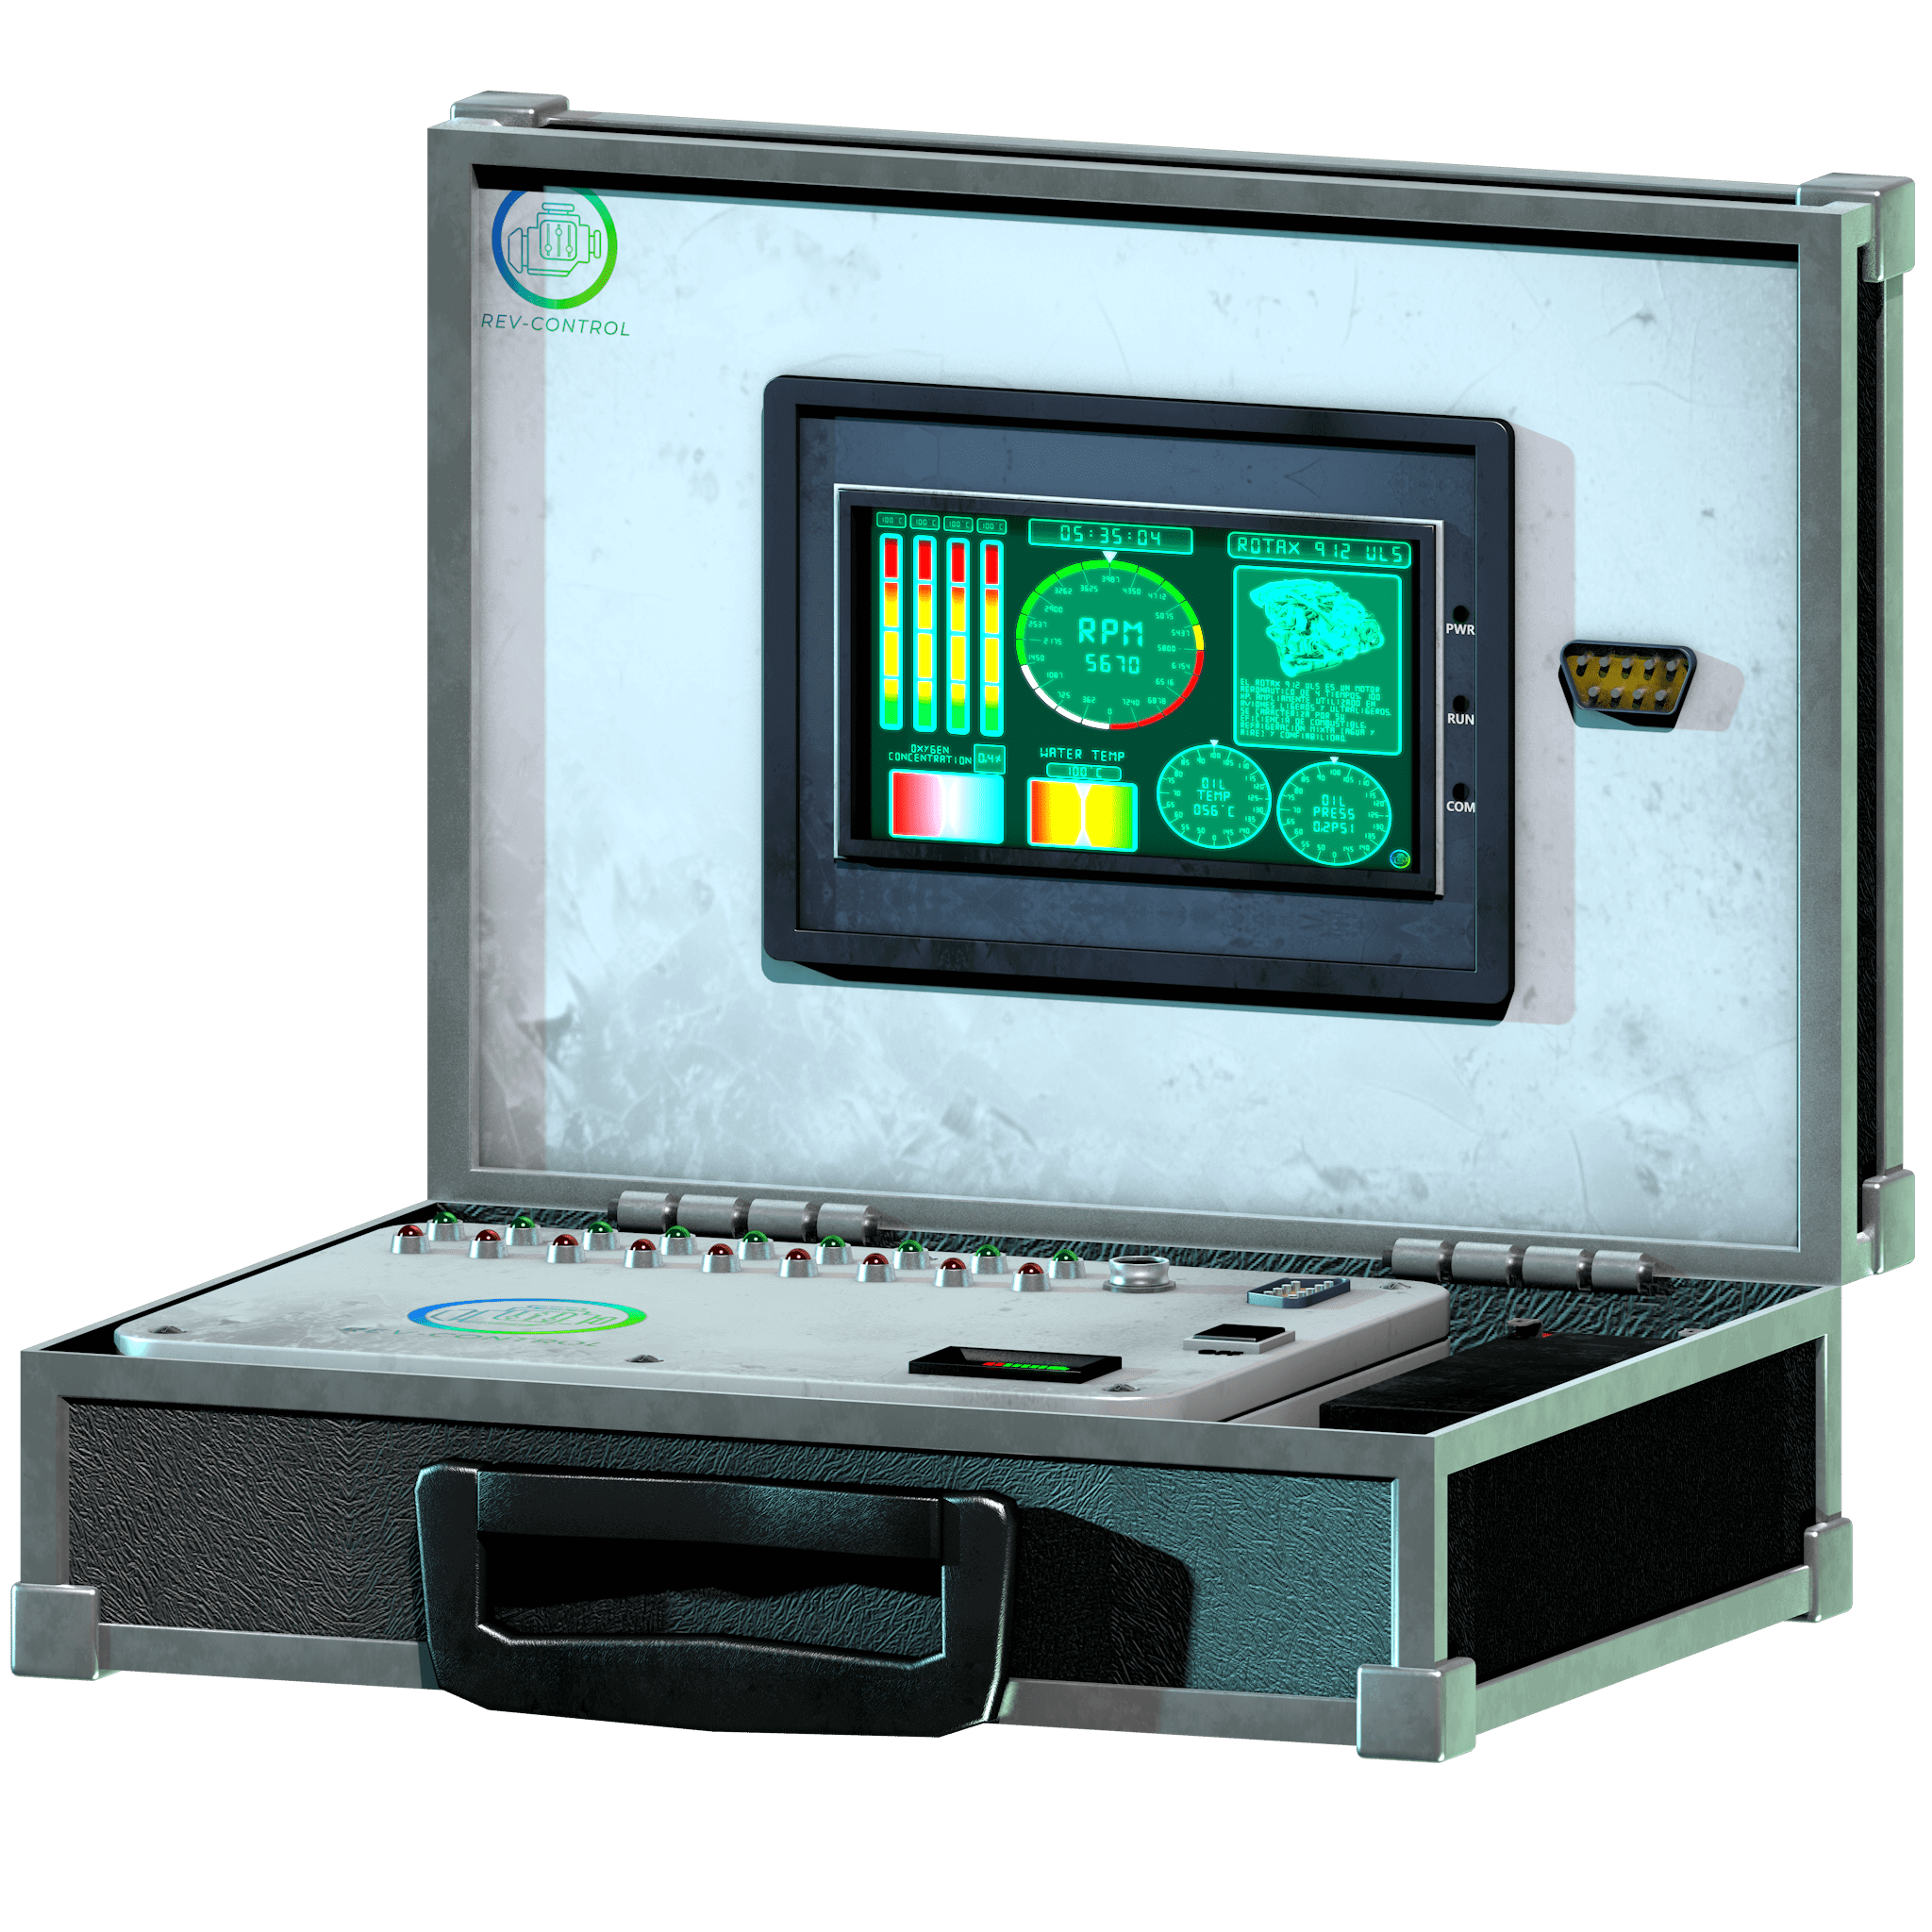
\includegraphics[width=0.6\textwidth]{Imagenes/Monitor y maletin-min.png}
    \caption{Imagen representativa del proyecto REV-CONTROL en funcionamiento.}
    \label{fig:representativa}
\end{figure}

\section{Diagrama en bloques del proyecto}

\begin{figure}[H]
    \centering
    \begin{tikzpicture}[
      block/.style={rectangle, draw, text centered, minimum height=1cm, minimum width=3cm, rounded corners},
      arrow/.style={-{Latex[length=3mm, width=2mm]}, thick},
      node distance=1.5cm
    ]
      
      % Definición de nodos
      \node[block, fill=cyan!30] (motor) {Motor en funcionamiento};
      \node[block, fill=green!30, below=of motor] (sensores) {Sensores de parámetros críticos};
      \node[block, fill=blue!30, below=of sensores] (condicionamiento) {Condicionamiento de señales};
      \node[block, fill=cyan!30, below=of condicionamiento] (lpc845) {Microcontrolador LPC845};
      \node[block, fill=green!30, below=of lpc845] (alarma) {Sistema de alarma};
      \node[block, fill=green!30, right=of lpc845] (monitor) {Monitor Kinseal};

      % Conexiones con flechas
      \draw[arrow] (motor) -- (sensores);
      \draw[arrow] (sensores) -- (condicionamiento);
      \draw[arrow] (condicionamiento) -- (lpc845);
      \draw[arrow] (lpc845) -- (alarma);
      \draw[arrow] (lpc845) -- (monitor);

    \end{tikzpicture}
    \caption{Diagrama en bloques del sistema REV-CONTROL.}
    \label{fig:diagrama_bloques}
\end{figure}

\section{Motor utilizado en el proyecto (ROTAX 912 ULS)}

El \textbf{\href{https://www.flyrotax.com/products/912-uls-s}{Rotax 912 ULS}} es un motor de cuatro tiempos ampliamente utilizado en aeronaves ligeras, vehículos todoterreno y aplicaciones industriales.  
\begin{itemize}
    \item Configuración: Motor bóxer de 4 cilindros, refrigerado por líquido y aire.  
    \item Cilindrada: 1,352 cm³.  
    \item Potencia: 100 HP (73.5 kW) a 5,800 RPM.  
    \item Alimentación: Sistema de carburadores duales.  
    \item Características destacadas: Alta fiabilidad, bajo peso, eficiencia de combustible y capacidad para operar con gasolina sin plomo.  
    \item Aplicación en el proyecto: Recolección y análisis de datos críticos como temperatura, presión de aceite, proporción aire-combustible y velocidad de rotación.  
\end{itemize}

\begin{figure}[H]
    \centering
    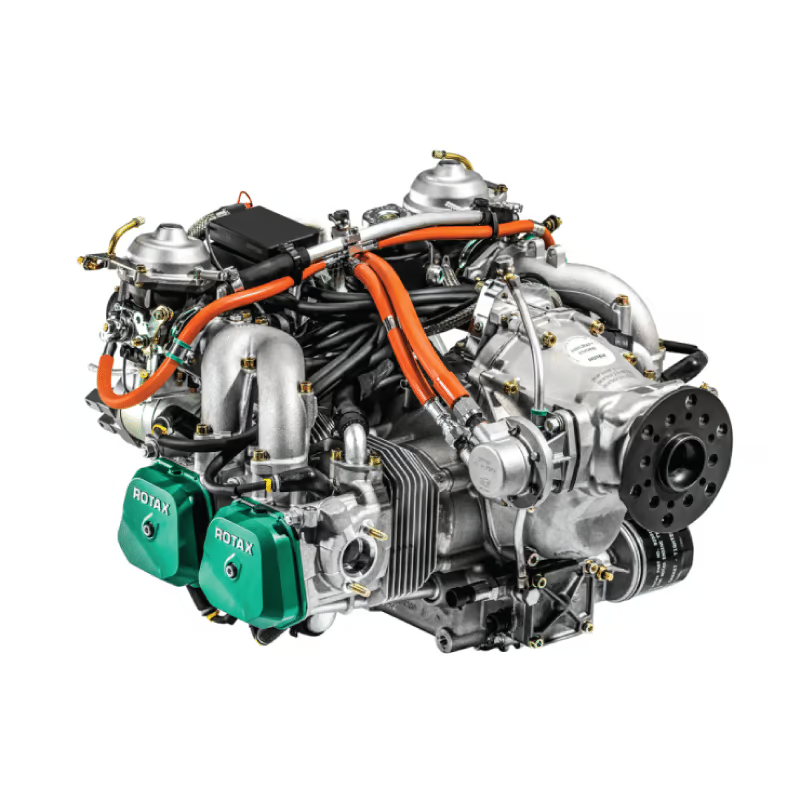
\includegraphics[width=0.8\textwidth]{Imagenes/ROTAX.png}
    \caption{Motor Rotax 912 ULS}
    \label{fig:motor_rotax_912}
\end{figure}


\section{Resultado conseguido}  
El resultado de \textbf{REV-CONTROL} es una herramienta integral para diagnóstico de motores, que ofrece mediciones precisas y en tiempo real de parámetros críticos. Su sistema permite a los técnicos obtener datos detallados de manera clara y sencilla, mejorando la eficacia en las reparaciones y mantenimiento de motores, además de ofrecer un sistema de alarmas para alertar de situaciones críticas en los parámetros monitoreados.
